% !TEX TS-program = pdflatex
% !TEX root = ../tesi.tex

%************************************************
\chapter{NASCITA DI UN PROTOTIPO}
\label{chp:nascita}
%************************************************

Possiamo ipotizzare, quindi , il computer come una mente bicamerale : un’entità
dotata di una spropositata  capacità logico-matematica, sicuramente superiore a
quella umana, che necessita, però, di un’altra entità che gli fornisca
dall’esterno  gli input necessari ad avviare il suo percorso  standardizzato
basato su una logica  «semplicemente» binaria: questa entità esterna è l’uomo.
Per dirla con Jaynes gli uomini possono  rappresentare  gli “dei” del computer:
la silenziosa “allucinazione sonora”  che guida e indirizza la “coscienza” digitale.

Storicamente si riscontra questo tipo di sequenza: lo strumento suona, il
computer elabora e  il suono elaborato viene diffuso dagli altoparlanti.

In questo modo però, il suono elaborato perde tutte le caratteristiche di
diffusione spaziale tipiche dello strumento acustico originale, in quanto
un altoparlante dispone di una sola direzione di diffusione del suono,.

Possiamo definire questa sequenza  un processo generato  nell’area
logico-matematica “geometrica” governata dall’emisfero sinistro.

L’idea generatrice di questo studio, invertendo inizialmente la sequenza
tradizionale, è quella di far diventare l’elaborazione L.E. “l’allucinazione
sonora”, il suono nascosto, che pervade un ipotetico “emisfero destro” dello
strumento acustico, in questo caso un flauto. È all’interno di questo emisfero,
dove sono racchiusi tutti i suoni non suonabili direttamente dalle chiavi dello
strumento, che si è concentrata la ricerca, esplorando nuovi timbri e  nuove
sonorità, uscendo così dai canoni classici dello strumento.

In tal modo è stato possibile sia restituire al suono elaborato, che dare  ai
suoni sintetici, le stesse caratteristiche di diffusione del suono acustico
facendo risuonare l’elaborazione L.E. dentro lo strumento.

Di conseguenza  viene annullato il divario spaziale tra suono L.E. e suono
acustico, essendo il flauto l’unica sorgente emissiva di suono.

Questo modo di diffusione potrà avere sia la funzione di generatrice di
sonorità, ma potrà anche essere usata parallelamente alla sequenza tradizionale,
in modo tale da non avere una sola direzione ma due che hanno come uscita
finale solamente lo strumento acustico.

Questo tipo di struttura sonora  permette di pensare il ”dispositivo” così
assemblato come   un unico strumento  che necessita della contemporanea
collaborazione di due persone: lo strumento in questo modo diventa un luogo di
incontro e collaborazione tra i due interpreti per la ricerca di nuove timbriche.

Come strumento da aumentare è stato scelto un flauto per due motivi: si voleva
lavorare sul flusso d’aria e il flauto è uno strumento a fiato non dotato di ancia.

Per realizzare questo  sistema era necessario immettere nel flauto un flusso di
onde di pressione generato dal live electronics.

Prima di giungere al dispositivo che ha restituito il risultato attualmente più
efficace sono stati elaborati una serie di prototipi.

Il primo passo è stato quello di analizzare un flauto studiandole sue
caratteristiche sia di emissione che strutturali.

Questa analisi si è concentrata soprattutto sulla testata del flauto in quanto l’onda prodotta doveva precedere l’imboccatura.
Tra l’imboccatura e la parte posteriore del flauto, chiusa da una ghiera, è collocato un tappo di sughero rimovibile. Questa è stata la zona su cui si è deciso di intervenire.

\begin{figure}
\centering
\subfloat[]
{
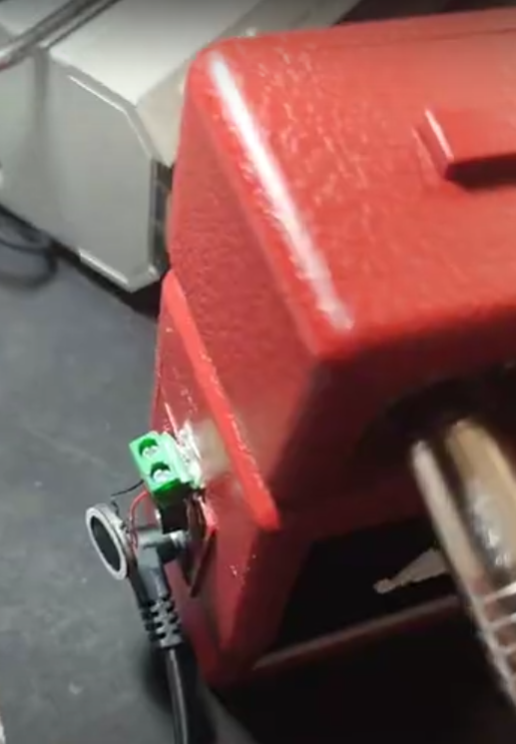
\includegraphics[width=.45\columnwidth]{Graphics/foto/alto.PNG}} \quad
\subfloat[]
{
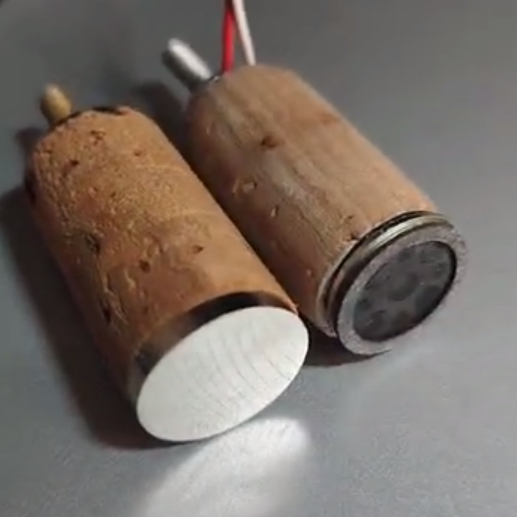
\includegraphics[width=.45\columnwidth]{Graphics/foto/tappo_parlante.PNG}}
\caption{Tappo Parlante}
\end{figure}

\section{Il tappo-parlante}

La prima idea è stato quello di convertire proprio il tappo di sughero in un altoparlante. Presa la misura del diametro interno del flauto, 18mm,si è cercato se nel mercato esistevano altoparlanti da 17mm. L’ altoparlante di questo diametro è di 1watt e 8 ohm. Per farlo suonare è stato usato un mini amplificatore per chitarra Marshall a cui era collegato di fabbrica  un altoparlante di diametro maggiore ma con le stesse caratteristiche. Tale altoparlante è stato scollegato ed è stato collegato il mini altoparlante di 17mm, con risultati sonori accettabili.

Il tappo da flauto è caratterizzato da un foro interno che permette il passaggio di una piccola asta filettata, dotata di testata di blocco, necessaria alla sua regolazione tramite la ghiera finale.
La prima idea è stata quella di forare il tappo  parallelamente al foro originario per far passare i cavi dell’altoparlante.
La parte del tappo verso l’imboccatura è stata scavata internamente in modo da poter consentire sia l’arretramento della testa della asta filettata, sia l’inserimento del mini altoparlante.
Per fare ciò è stato necessario sostituire l’asta filettata originale con una vite che avesse una testa di diametro inferiore al diametro del tappo. In questo momento sembrava ancora necessario mantenere la possibilità di regolazione dell’altezza del tappo all’interno della testata del flauto.
Logicamente questo progetto ha comportato la necessita di forare la ghiera di regolazione in due punti per far passare i cavi.

Nella foto è possibile vedere il confronto tra un tappo originale della testata di un flauto e d il tappo elaborato per questo prototipo.

La fisionomia dell’altoparlante è stato il problema di questo prototipo.
Infatti il suono di questo altoparlante non è prodotto tramite l’oscillazione di un corpo ma bensì dalla messa in vibrazione di cristalli. Tale vibrazione non è in grado di  produrre uno spostamento d’aria dentro la canna del flauto anche a causa del ridottissimo diametro dell’altoparlante. Oltretutto il suono prodotto dall’altoparlante era completamente dal suono del flautista ed essendo così piccolo l’altoparlante aveva una risposta che non contemplava minimamente le basse frequenze.

\begin{figure}
\centering
{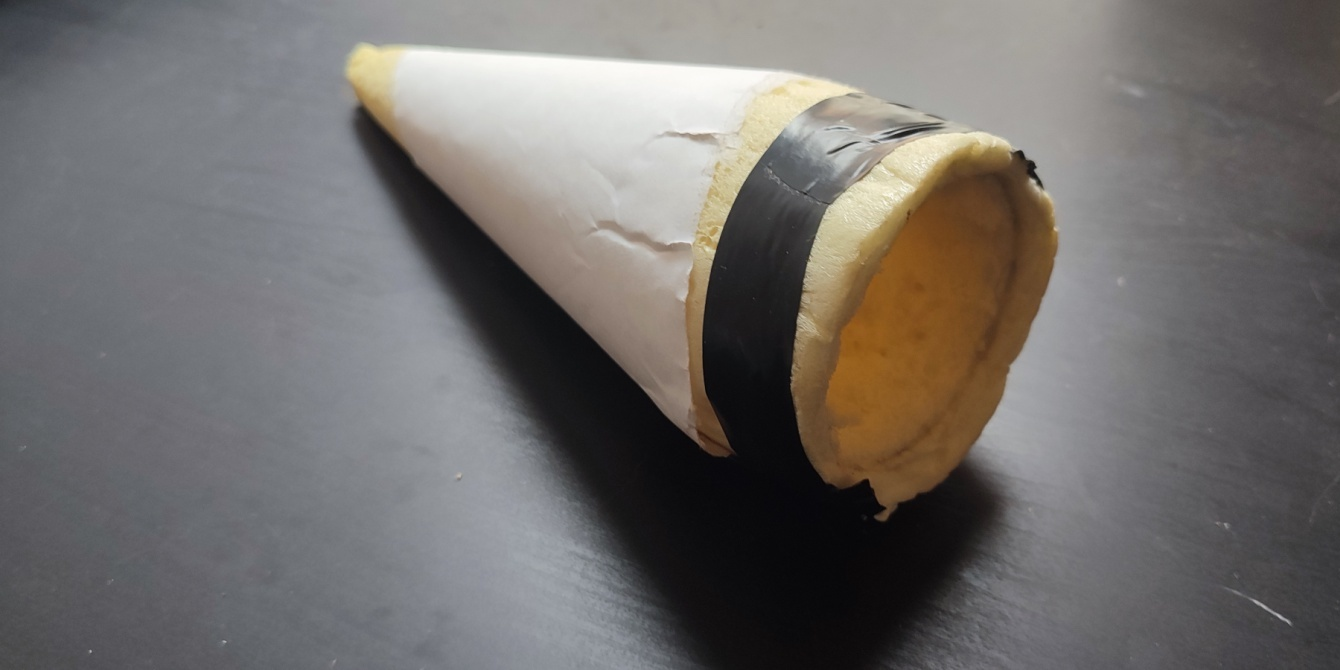
\includegraphics[width=.98\columnwidth]{Graphics/foto/schiuma}}
\caption{Cono di Schiuma}
\label{fig:schiuma}
\end{figure}

\section{Il cono di schiuma}

Dopo il fallimento del tappo-parlante è stato necessario cambiare l’approccio  progetto.

In un flauto l’elemento principale che genera suono è la colonna d’aria in movimento. Questa colonna d’aria, cambiando diteggiatura, cambia lunghezza e di conseguenza cambia l’intonazione.
Era necessario, quindi, per mettere in movimento la colonna d’aria del flauto un altoparlante di dimensioni notevolmente superiori a quelle del tappo-parlante.
Il primo tentativo di convogliare un flusso d’aria dentro il flauto fu realizzato tramite un cono di schiuma espansa, internamente cavo, collegato da una parte con un altoparlante di 7cm di diametro e dall’altra con la testata del flauto a cui era stato tolto il tappo interno. Logicamente l’altoparlante era collegato ad un amplificatore a cui arrivavano segnali generati da un computer.

Il problema principale di questo prototipo era soprattutto l’instabilità del sistema creata da peso dal peso dell’altoparlante. Parallelamente nacque il

proposito di poter sfruttare dia la parte positiva che negativa della vibrazione della membrana dell’altoparlante.



\section{Il primo imbuto}

\begin{figure}
\centering
\subfloat[]
{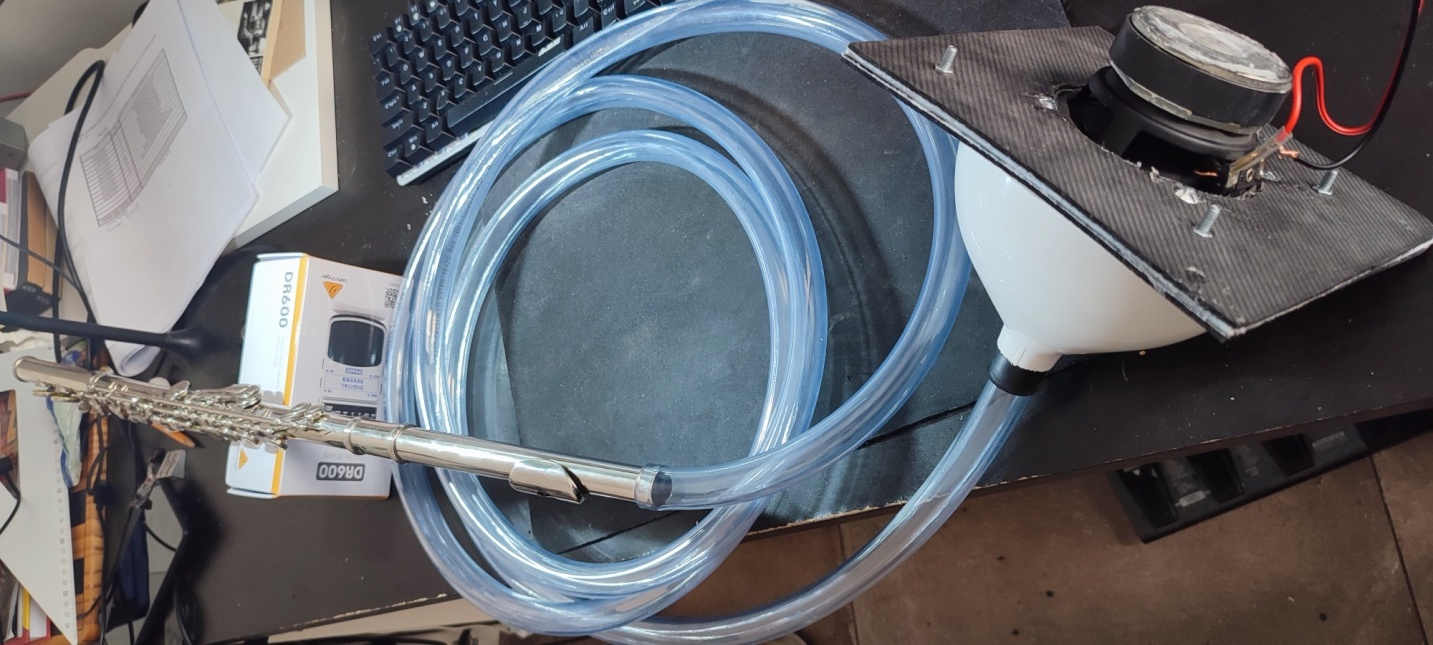
\includegraphics[width=.99\columnwidth]{Graphics/foto/imbuto1}} \\
\subfloat[]
{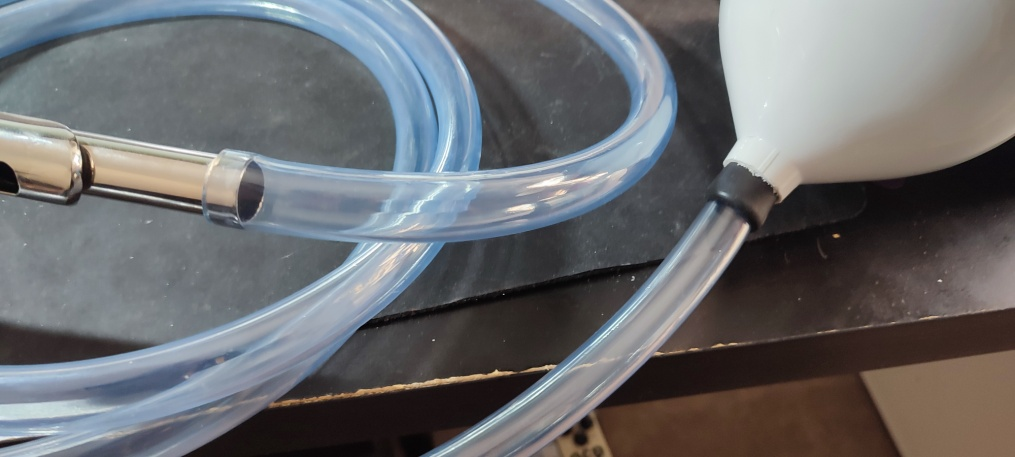
\includegraphics[width=.99\columnwidth]{Graphics/foto/imbuto2}}
\end{figure}

Vista la fragilità strutturale del cono di spugna si è pensato di sostituire il
collegamento tra l’altoparlante e il flauto con un imbuto collegato al flauto tramite un tubo di gomma.  Il collegamento tra l’imbuto e il tubo è stato
realizzato tramite un gommino antiscivolo per sedie forato, in grado di compensare la differenza di diametro tra il foro dell’imbuto e il tubo di gomma.

Per questo prototipo è stato scelto un tubo di gomma con il dimetro interno identico al diametro esterno del flauto in modo da poter realizzare un incastro.
Per raccordare l’altoparlante all’imbuto è stata usata una lastra di plexiglass rivestita da entrambi i lati due tappetini per il mouse forati con funzione di guarnizione. Inizialmente si è pensato di posizionare l’altoparlante da un

lato della lastra e l’imbuto dall’altra. Successivamente, come da foto, sia l’altoparlante che l’imbuto sono stati montati dallo stesso lato della lastra.
Il flusso all’interno del flauto, però, risultava ancora debole per cui si è pensato di sfruttare sia la fase positiva che quella negativa della membrana dell’altoparlante.

\begin{figure}%[t!]
\centering
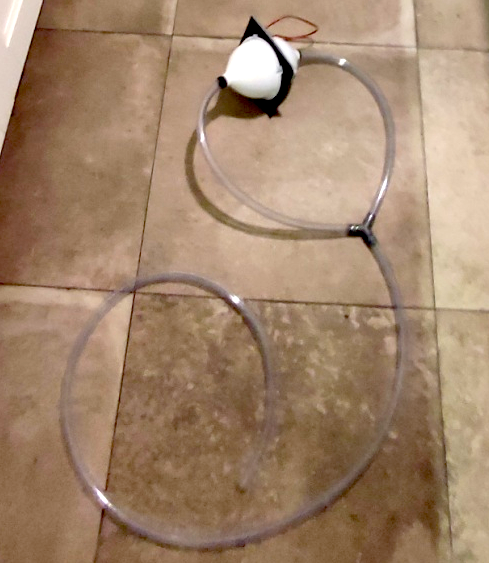
\includegraphics[width=0.99\columnwidth]{Graphics/foto/biconico}
%\caption[]{Magnetic Resonator Piano.\\ Electromagnetically augmented grand piano}
%\label{mrp}
\end{figure}

\section{Il Biconico}

Vista la presenza delle guarnizioni sulle due facciate della lastra si è pensato di montare un secondo imbuto identico al precedente sul retro l’altoparlante.

I due tubi convergono a metà percorso in un unico tubo, che si collega alla testata del flauto, tramite un raccordo Y.
Il flusso derivante da questo nuovo tentativo risultò ancora insufficiente ad innescare la colonna d, aria all’interno del flauto.

Tale mancanza di flusso venne imputata alla dimensione ridotta dell’altoparlante e quindi venne progettato un sistema identico con un altoparlante di 5 pollici di diametro.
Inoltre i due imbuti non erano sufficienti  schermare verso l’esterno le sonorità generate dall’altoparlante.

\begin{figure}[ht!]
\centering
\subfloat[]
{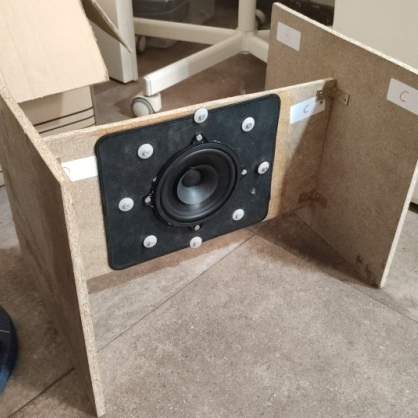
\includegraphics[width=.45\columnwidth]{Graphics/foto/scatola1}} \quad
\subfloat[]
{\label{fig:example-b}%
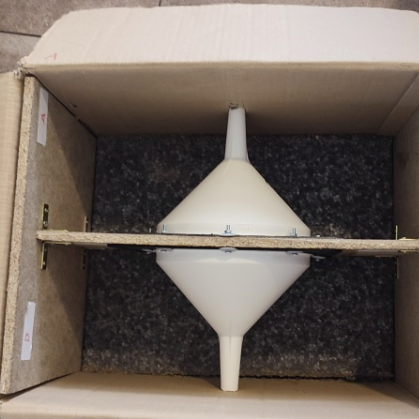
\includegraphics[width=.45\columnwidth]{Graphics/foto/scatola2}} \\
\subfloat[]
{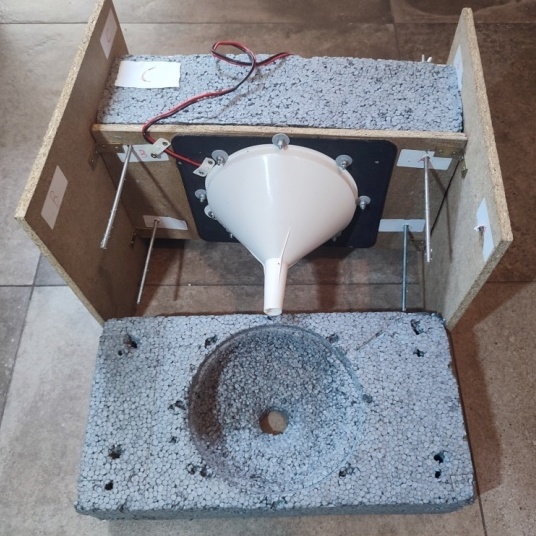
\includegraphics[width=.45\columnwidth]{Graphics/foto/scatola3}} \quad
\subfloat[]
{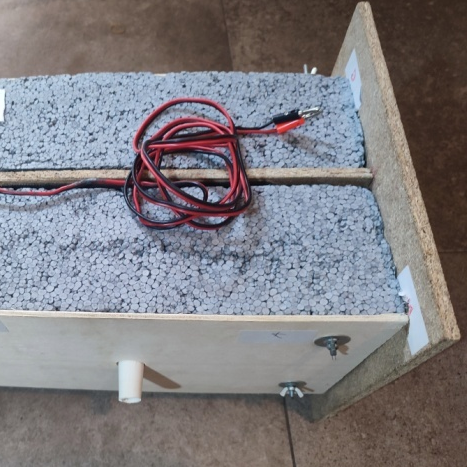
\includegraphics[width=.45\columnwidth]{Graphics/foto/scatola4}}
\caption{Scatola per il biconico}
\label{fig:scatola}
\end{figure}

\section{La Scatola}

Con lo stesso procedimento l’altoparlante da cinque pollici e due nuovi  imbuti di diametro adeguato sono stati montati su una lastra di legno.
Con la previsione di dover insonorizzare quanto prodotto dall’altoparlante  si è pensato ad un supporto a forma di H in grado di poter essere inserito in una scatola di cartone il cui fondo era foderato di polistirolo [Fig. \ref{fig:scatola}].

Il rettangolo di polistirolo è stato sagomato in modo tale da permettere l’inserimento dei supporti verticali tra la parete della scatola e la stessa tavoletta di polistirolo.

Per l’insonorizzazione dei due imbuti si è provveduto a scavare  all’interno di una tavola di polistirolo  un volume simile al negativo dell’imbuto.
Per ricavare una sagoma adatta è stato foderato un imbuto con un foglio di carta vetrata  a grana grossa  in modo tale che pressando e ruotando  questo imbuto sul polistirolo si è scavata la relativa sagoma [Fig. \ref{fig:scatola}].


Per l’applicazione dei pannelli di polistirolo laterali alla struttura ad H, si è fatto ricorso a quattro barre filettate passanti  e due  tavolette di legno.  Le tavolette di legno sono state applicate mediante dei dadi a farfalla  in modo da far aderire la tavolette sul polistirolo e di conseguenza sugli imbuti [Fig. \ref{fig:scatola}].

L’insonorizzazione si è completata inserendo un coperchio di polistirolo con al centro delle sagomature per farlo coincidere con la parte superiore della struttura ad H.

Si è ipotizzato che la mancanza di un elevato flusso all’interno del flauto dipendesse dalla scarsa velocità del flusso stesso determinata dalla  sezione del tubo di gomma usato. È stato necessario, quindi, progettare un raccordo in grado di collegare il diametro del foro dell’imbuto con il ridotto diametro del nuovo tubo. Nuovamente sono stati usati i gommini antiscivolo per sedie.

È stato possibile infatti inserire nella parete del gommino l’elemento in plastica di uno stop a cui era stata tagliata la  parte finale. Questo è stato possibile in quanto il diametro esterno  della parte in plastica dello stop si adattava perfettamente ai 7mm del diametro interno del nuovo tubo. Un tubo di diametro ridotto ha permesso di entrare direttamente nella testata del flauto e collegarsi al tappo tramite l’inserimento all’interno del tappo stesso  di una identica parte in plastica di stop [Fig. \ref{fig:scatola}].

\begin{figure}[t!]
\centering
\subfloat[]
{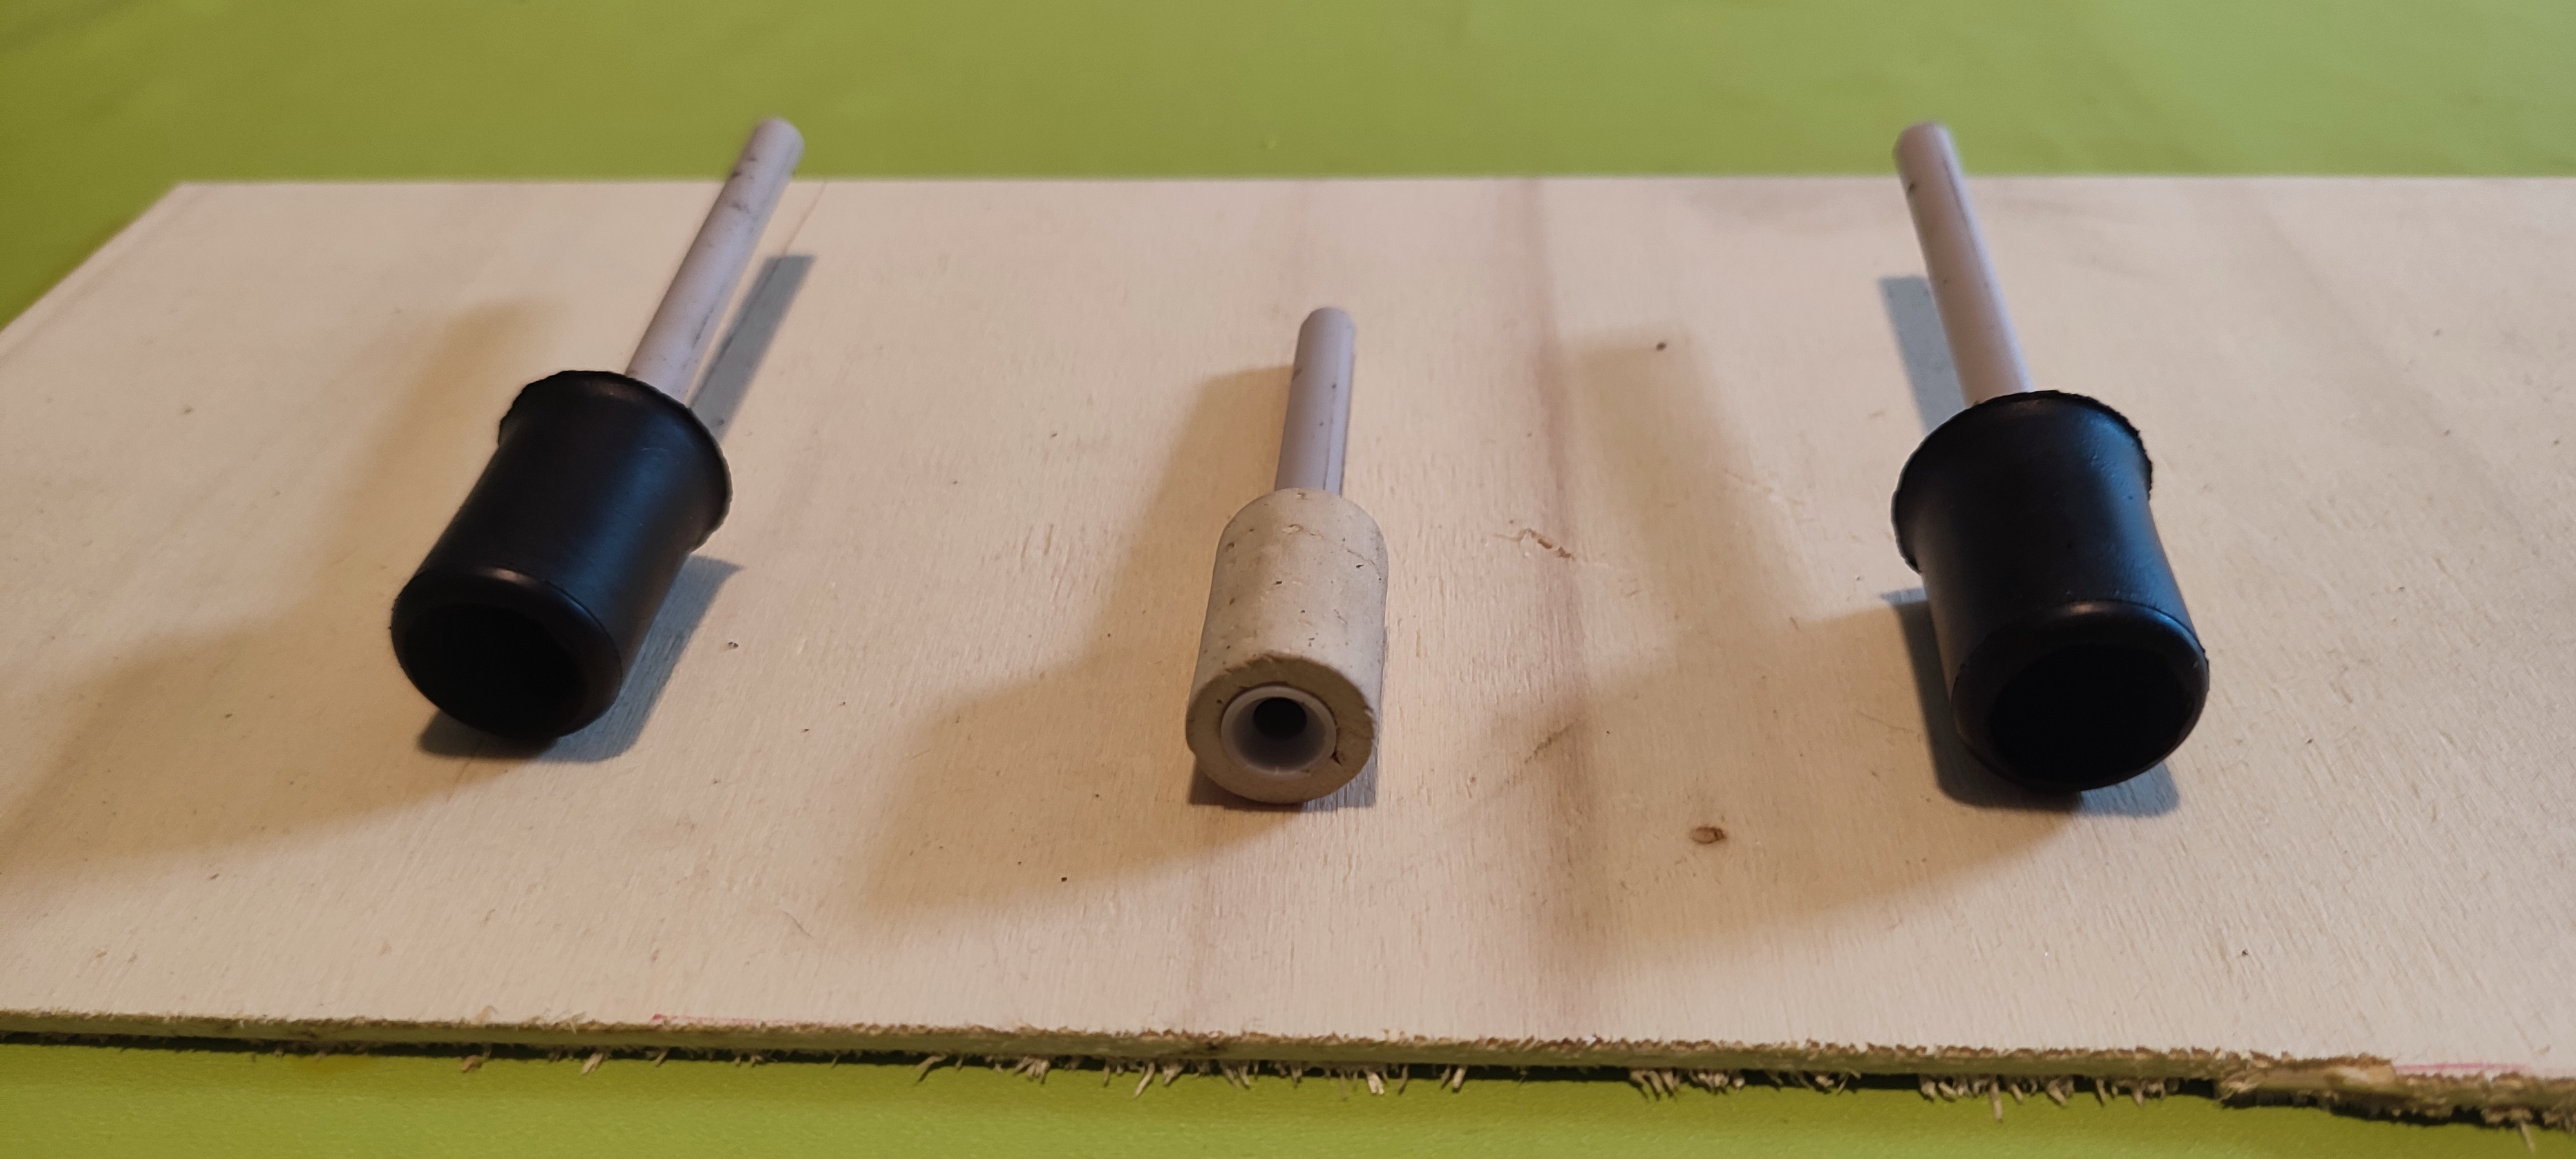
\includegraphics[width=.99\columnwidth]{Graphics/foto/1694686916414}} \\
\subfloat[]
{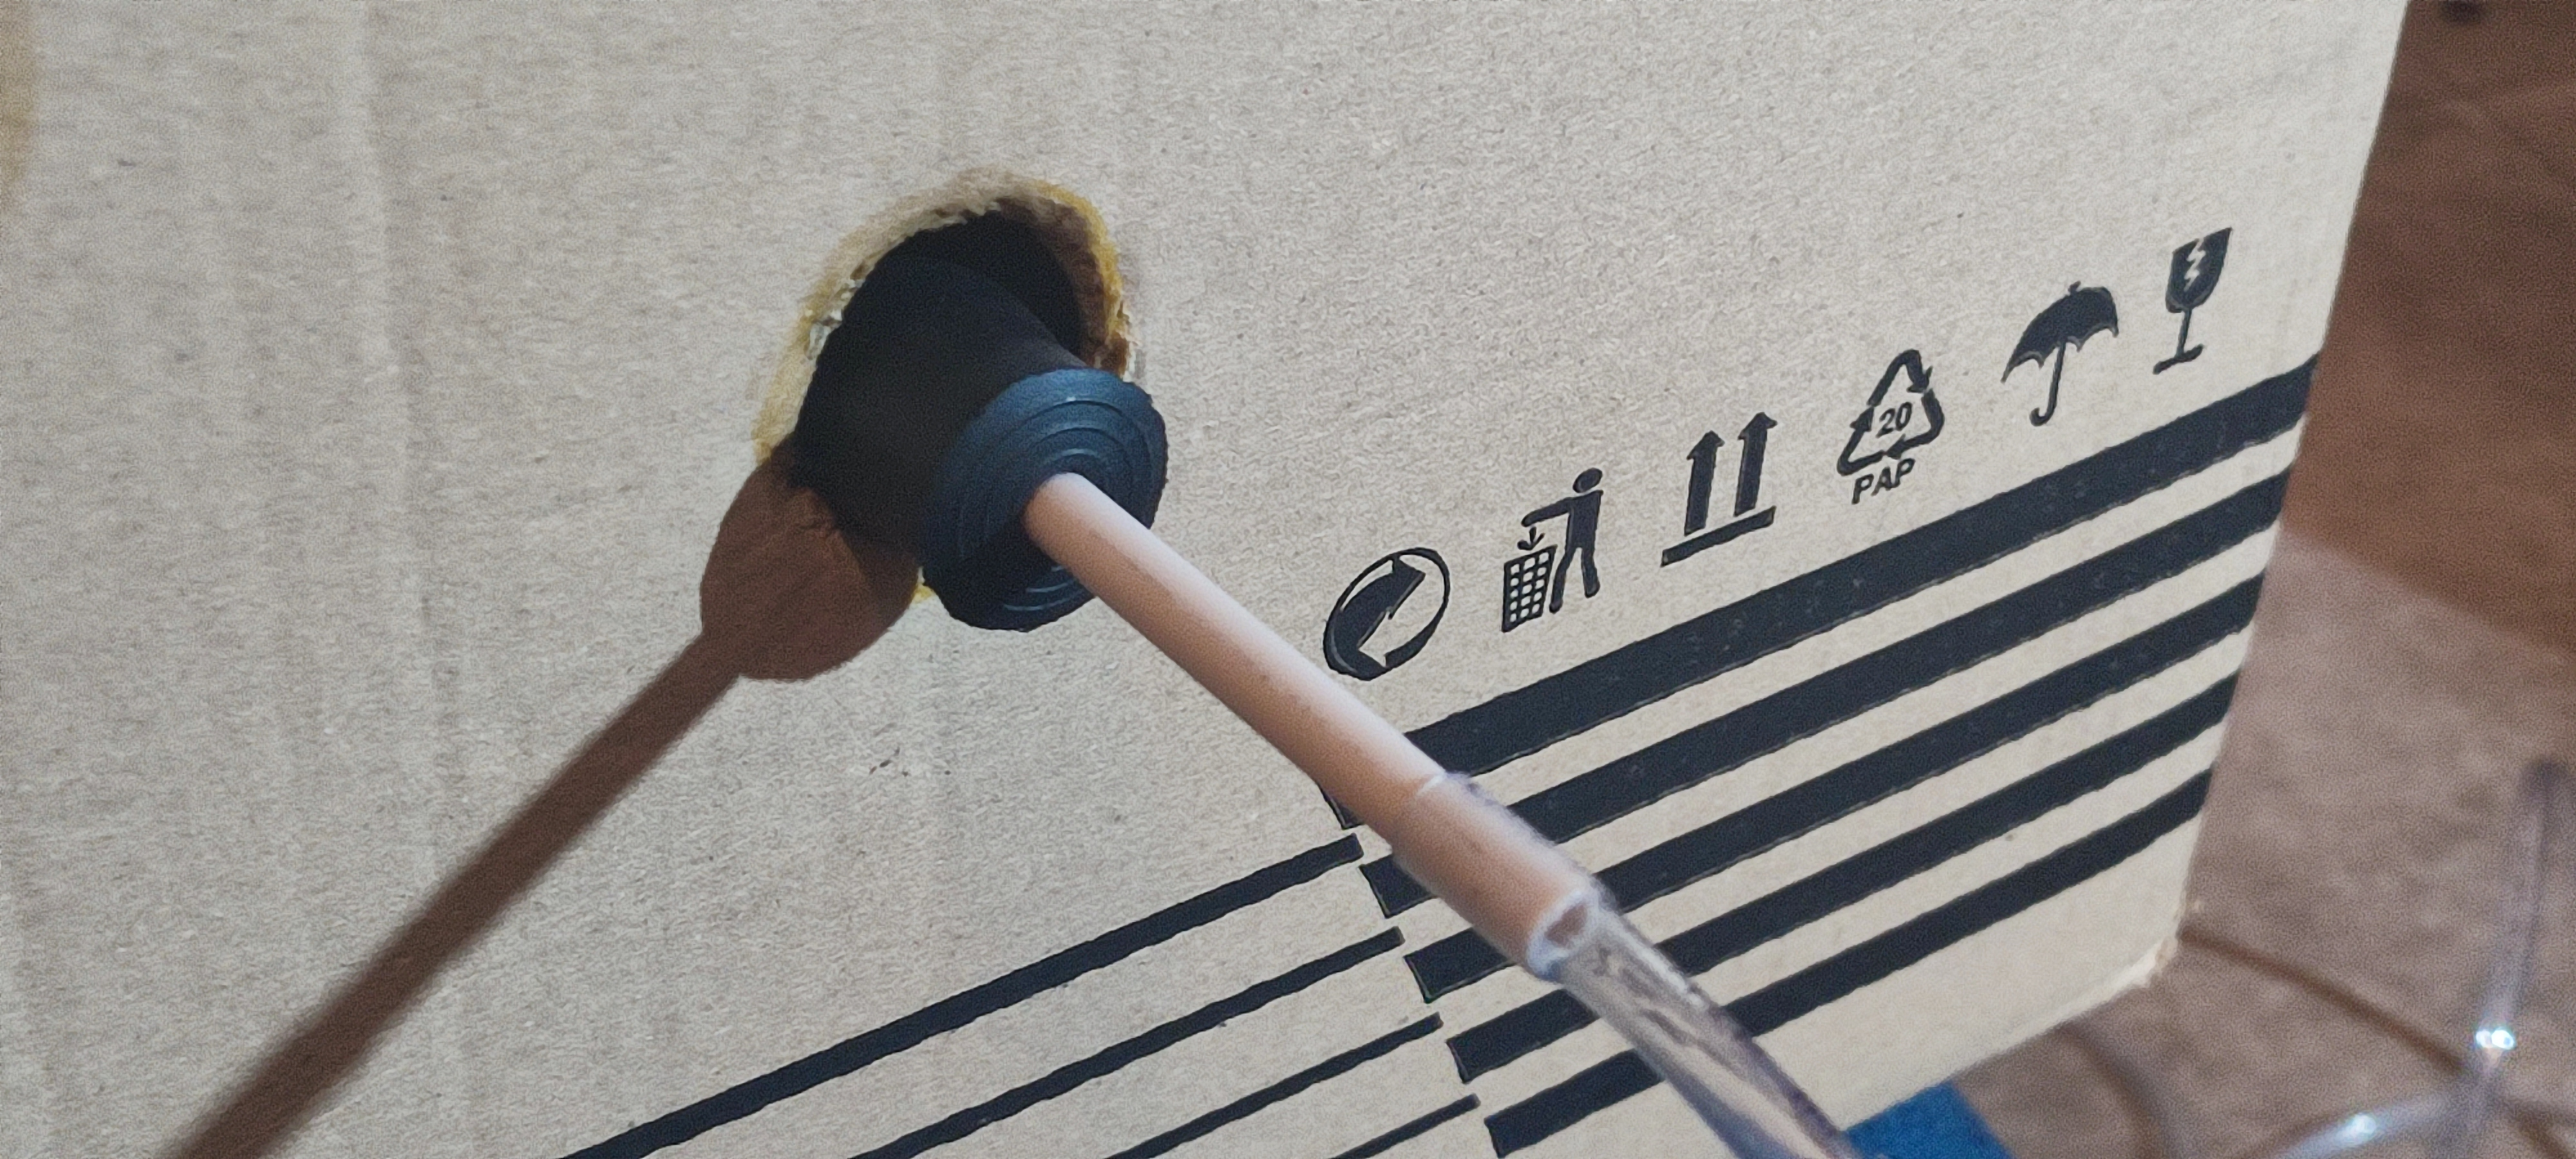
\includegraphics[width=.99\columnwidth]{Graphics/foto/1697469349089}}
\caption{Riduttori di pressione}
\label{fig:example}
\end{figure}

I due tubi collegati agli imbuti si collegano al tubo che entra dentro al flauto con un collegamento a $Y$ simile al precedente “biconico” ma di diametro ridotto.

Rendendo operativo questo muovo sistema (collegamento computer, amplificatore, altoparlante, flauto) nuovamente venne riscontrato uno scarso flusso all’interno del flauto. Tale mancanza di flusso era determinata da due fattori:

\begin{enumerate}
  \item Il doppio flusso teorizzato in realtà tendeva a zero in quanto il flusso positivo generato dello spostamento della membrana era annullato dal contemporaneo spostamento negativo della membrane stessa.
  \item L’effetto desiderato all’interno del tubo del flauto non dipendeva dalla         velocità del flusso determinata dalla ristretta sezione del tubo di gomma ma dalla pressione dell’aria all’interno del tubo stesso.
\end{enumerate}

Da queste considerazioni si è deciso sia di utilizzare solo la parte positiva dello spostamento della membrana dell’altoparlante che di aumentare il diametro del tubo di gomma in modo da accrescere la pressione del flusso.
Queste scelte consentivano tecnicamente di poter usare un altoparlante più grande in modo da sfruttare il più possibile l’aumentata pressione del flusso.

\section{Il Flauto Bicamerale}

Per generare un flusso adeguato è stato adottato un altoparlante subwoofer da 8 pollici, diametro esterno di $21 cm$, con una potenza di $300 Watt$ e con un’impedenza di $4 \Omega$:

Come contenitore è stato scelto un imbutone per lo smaltimento dei calcinacci in pvc composto da un cilindro attaccato a un tronco di cono.
Il diametro del cilindro è di $21,7 cm$ di poco superiore ai $21 cm$ del diametro esterno dell’altoparlante [Fig. \ref{fig:imbutone}].

\begin{figure}
\centering
\subfloat[]
{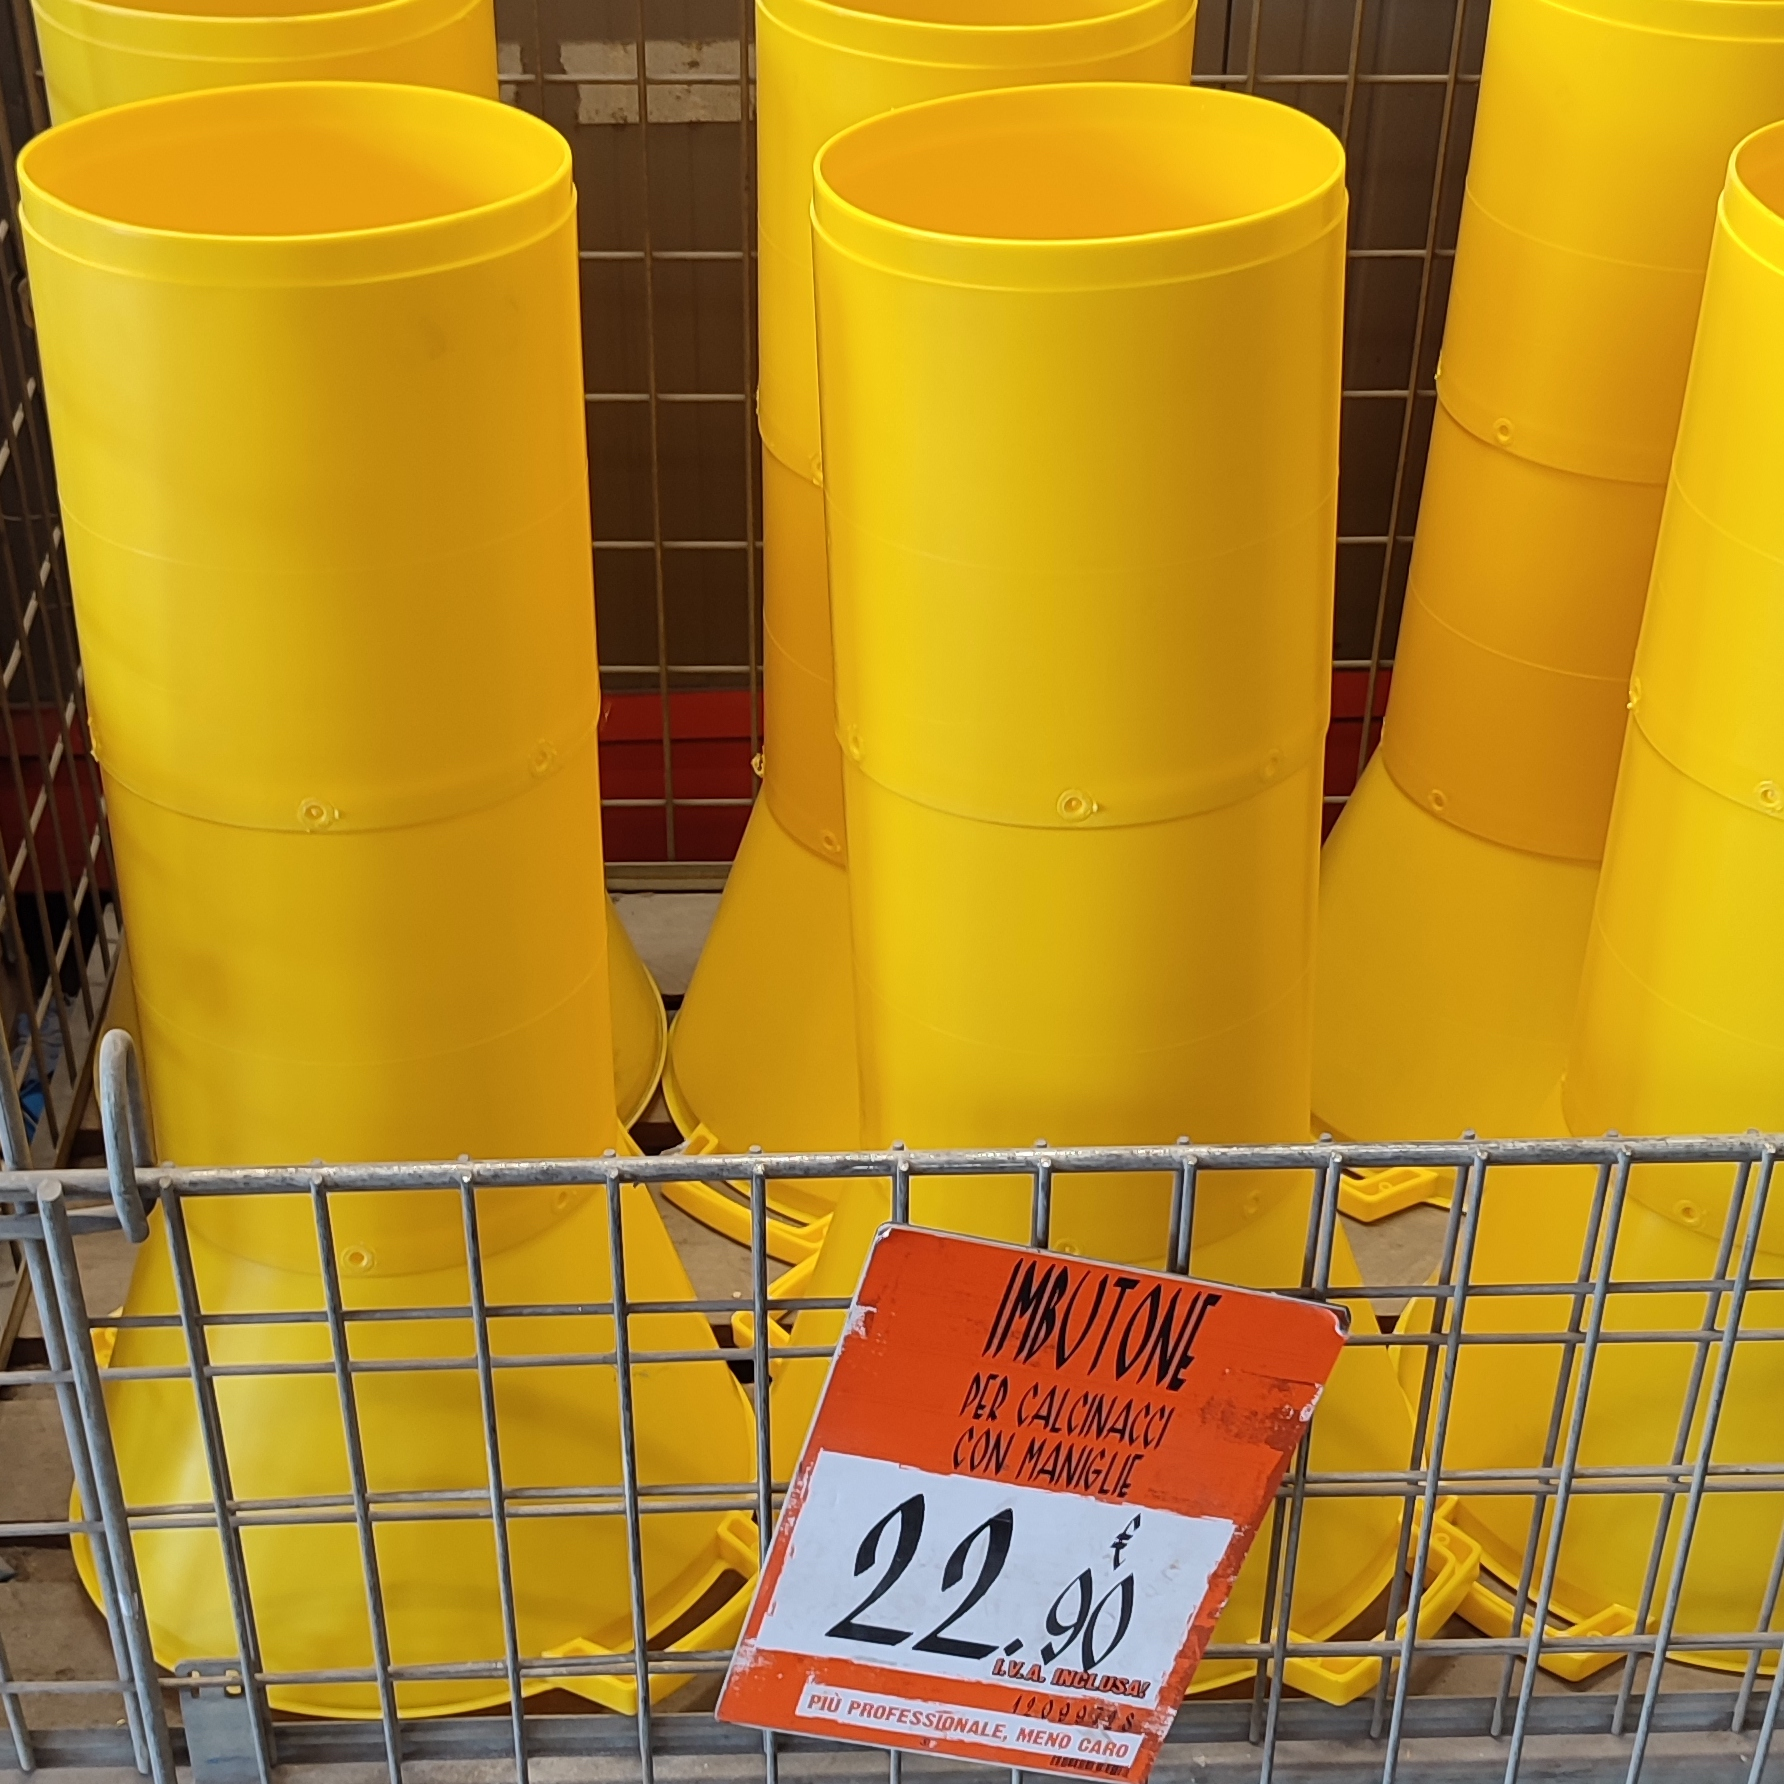
\includegraphics[width=.45\columnwidth]{Graphics/foto/1697454976316}} \quad
\subfloat[]
{
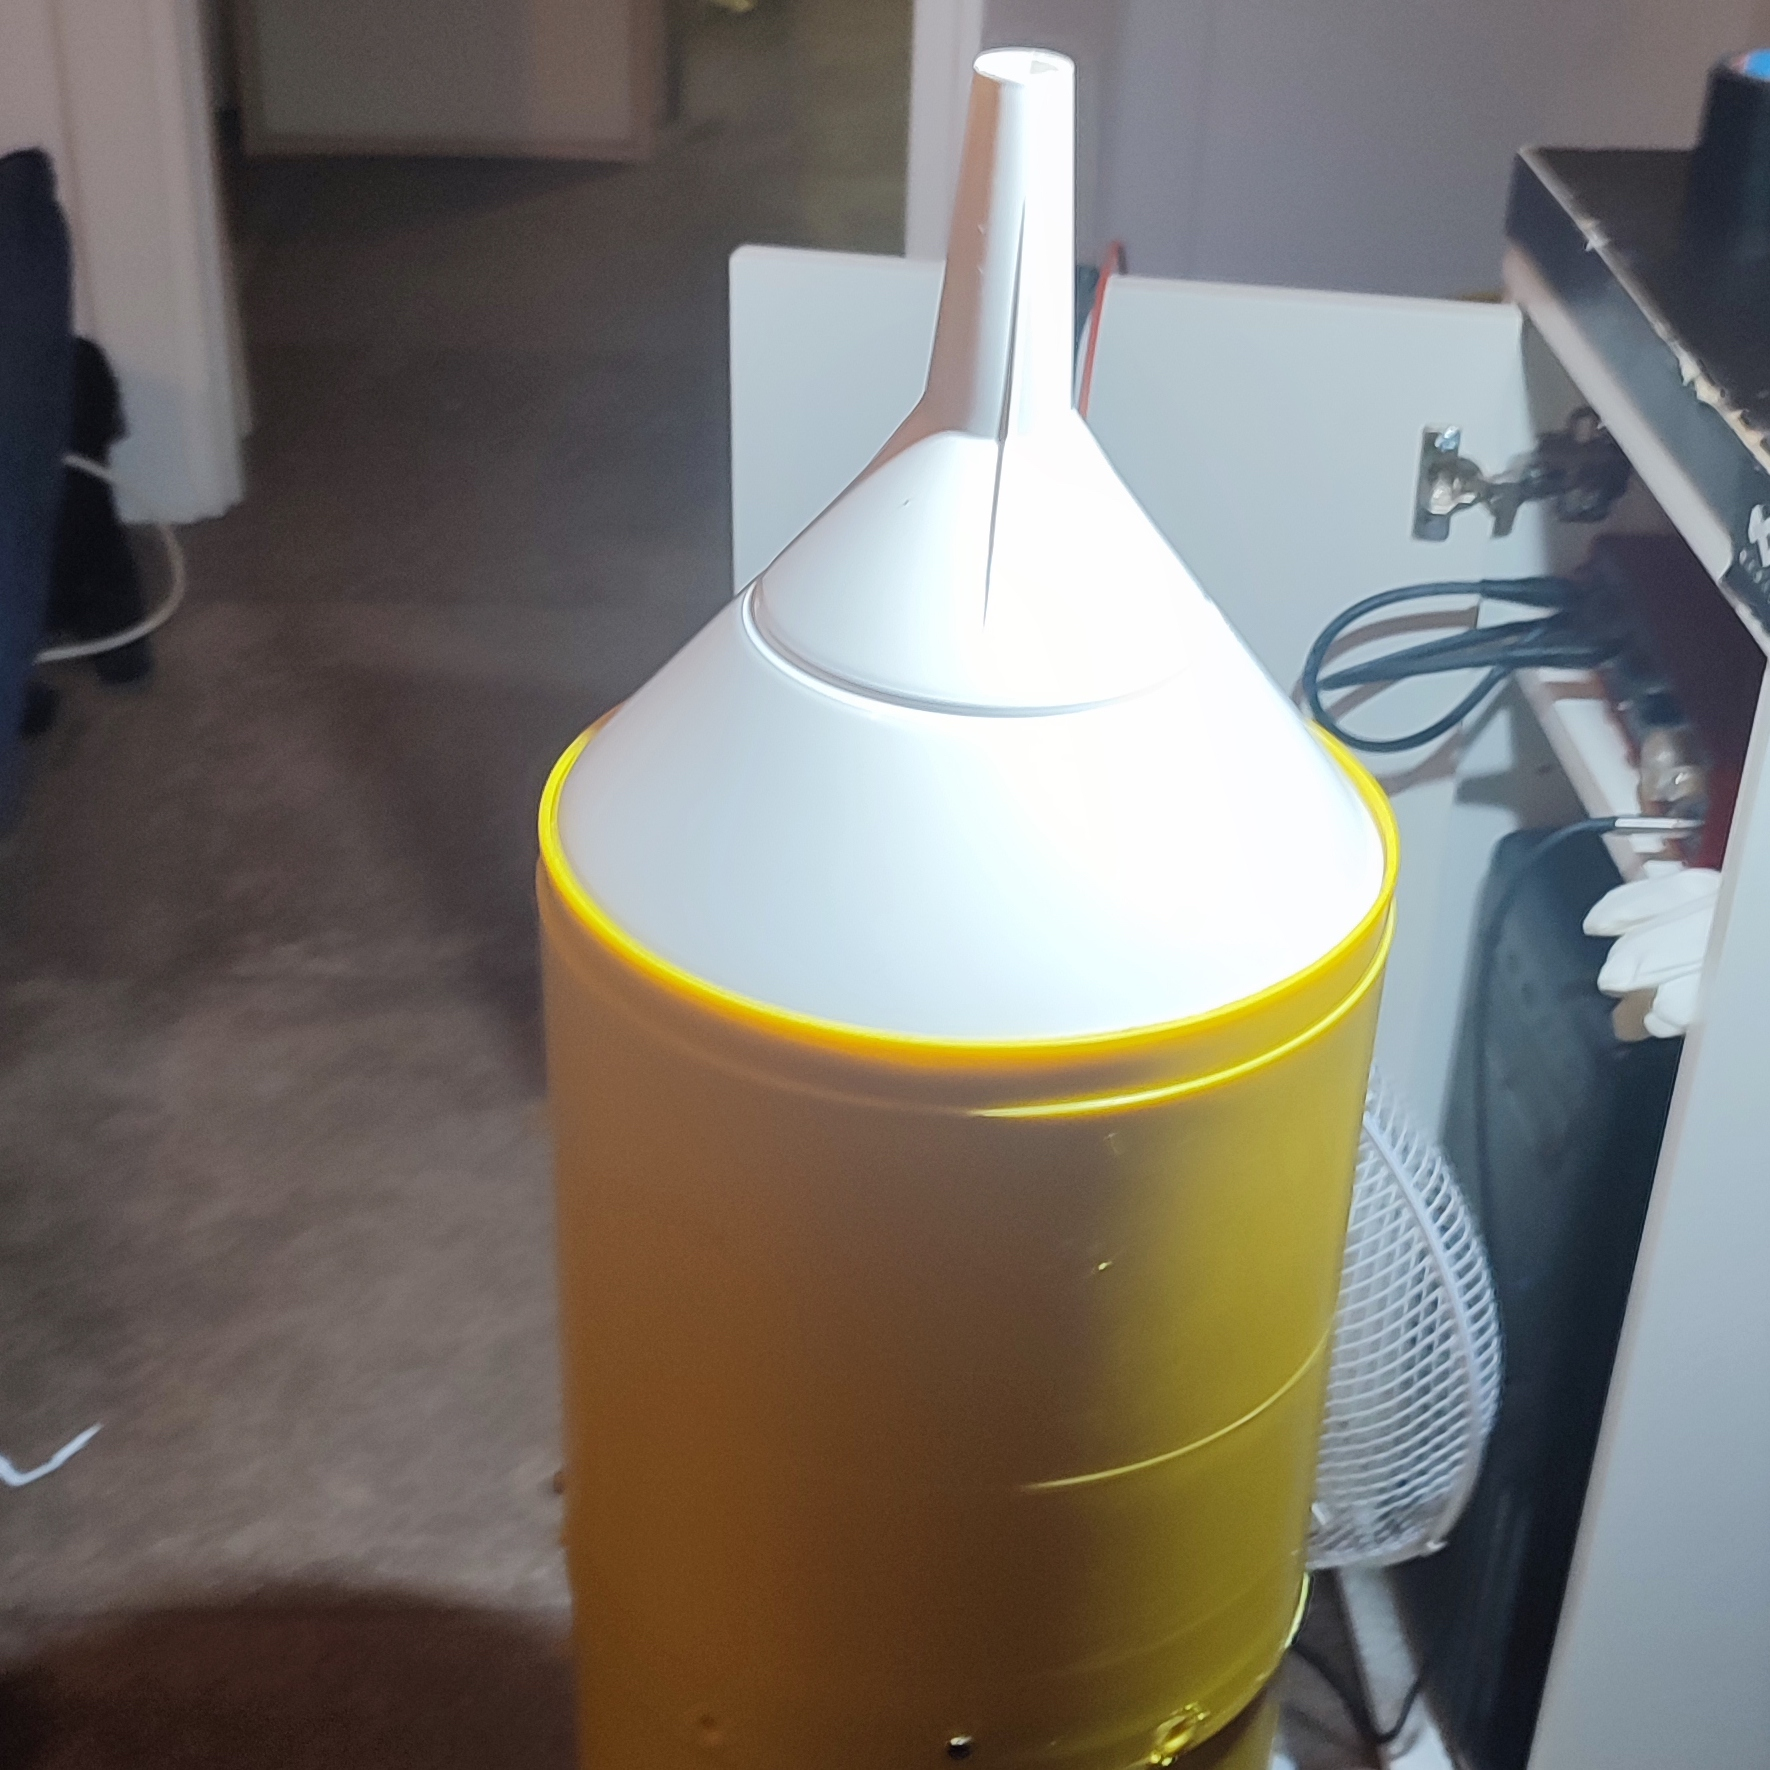
\includegraphics[width=.45\columnwidth]{Graphics/foto/1697454976170}} \\
\subfloat[]
{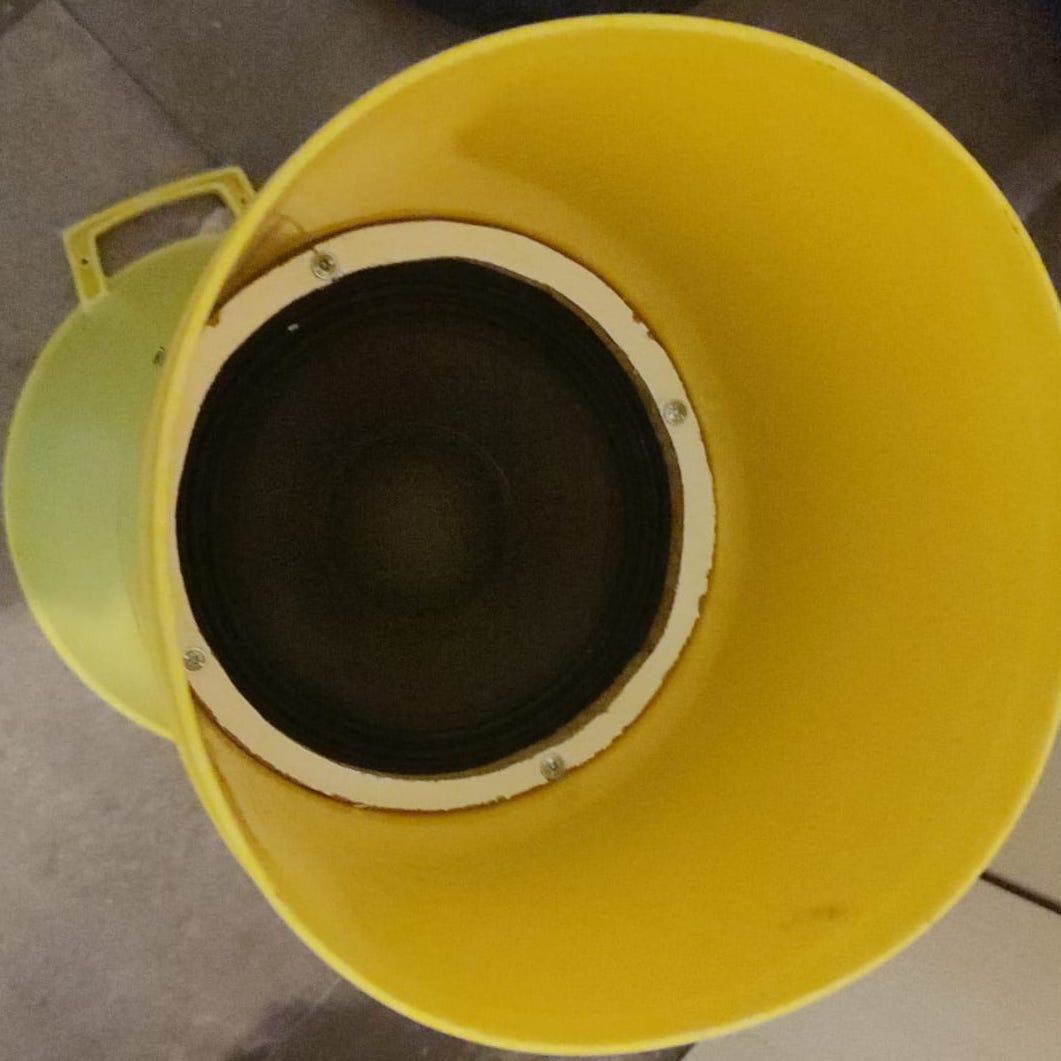
\includegraphics[width=.45\columnwidth]{Graphics/foto/IMG-20230925-WA0002}} \quad
\subfloat[]
{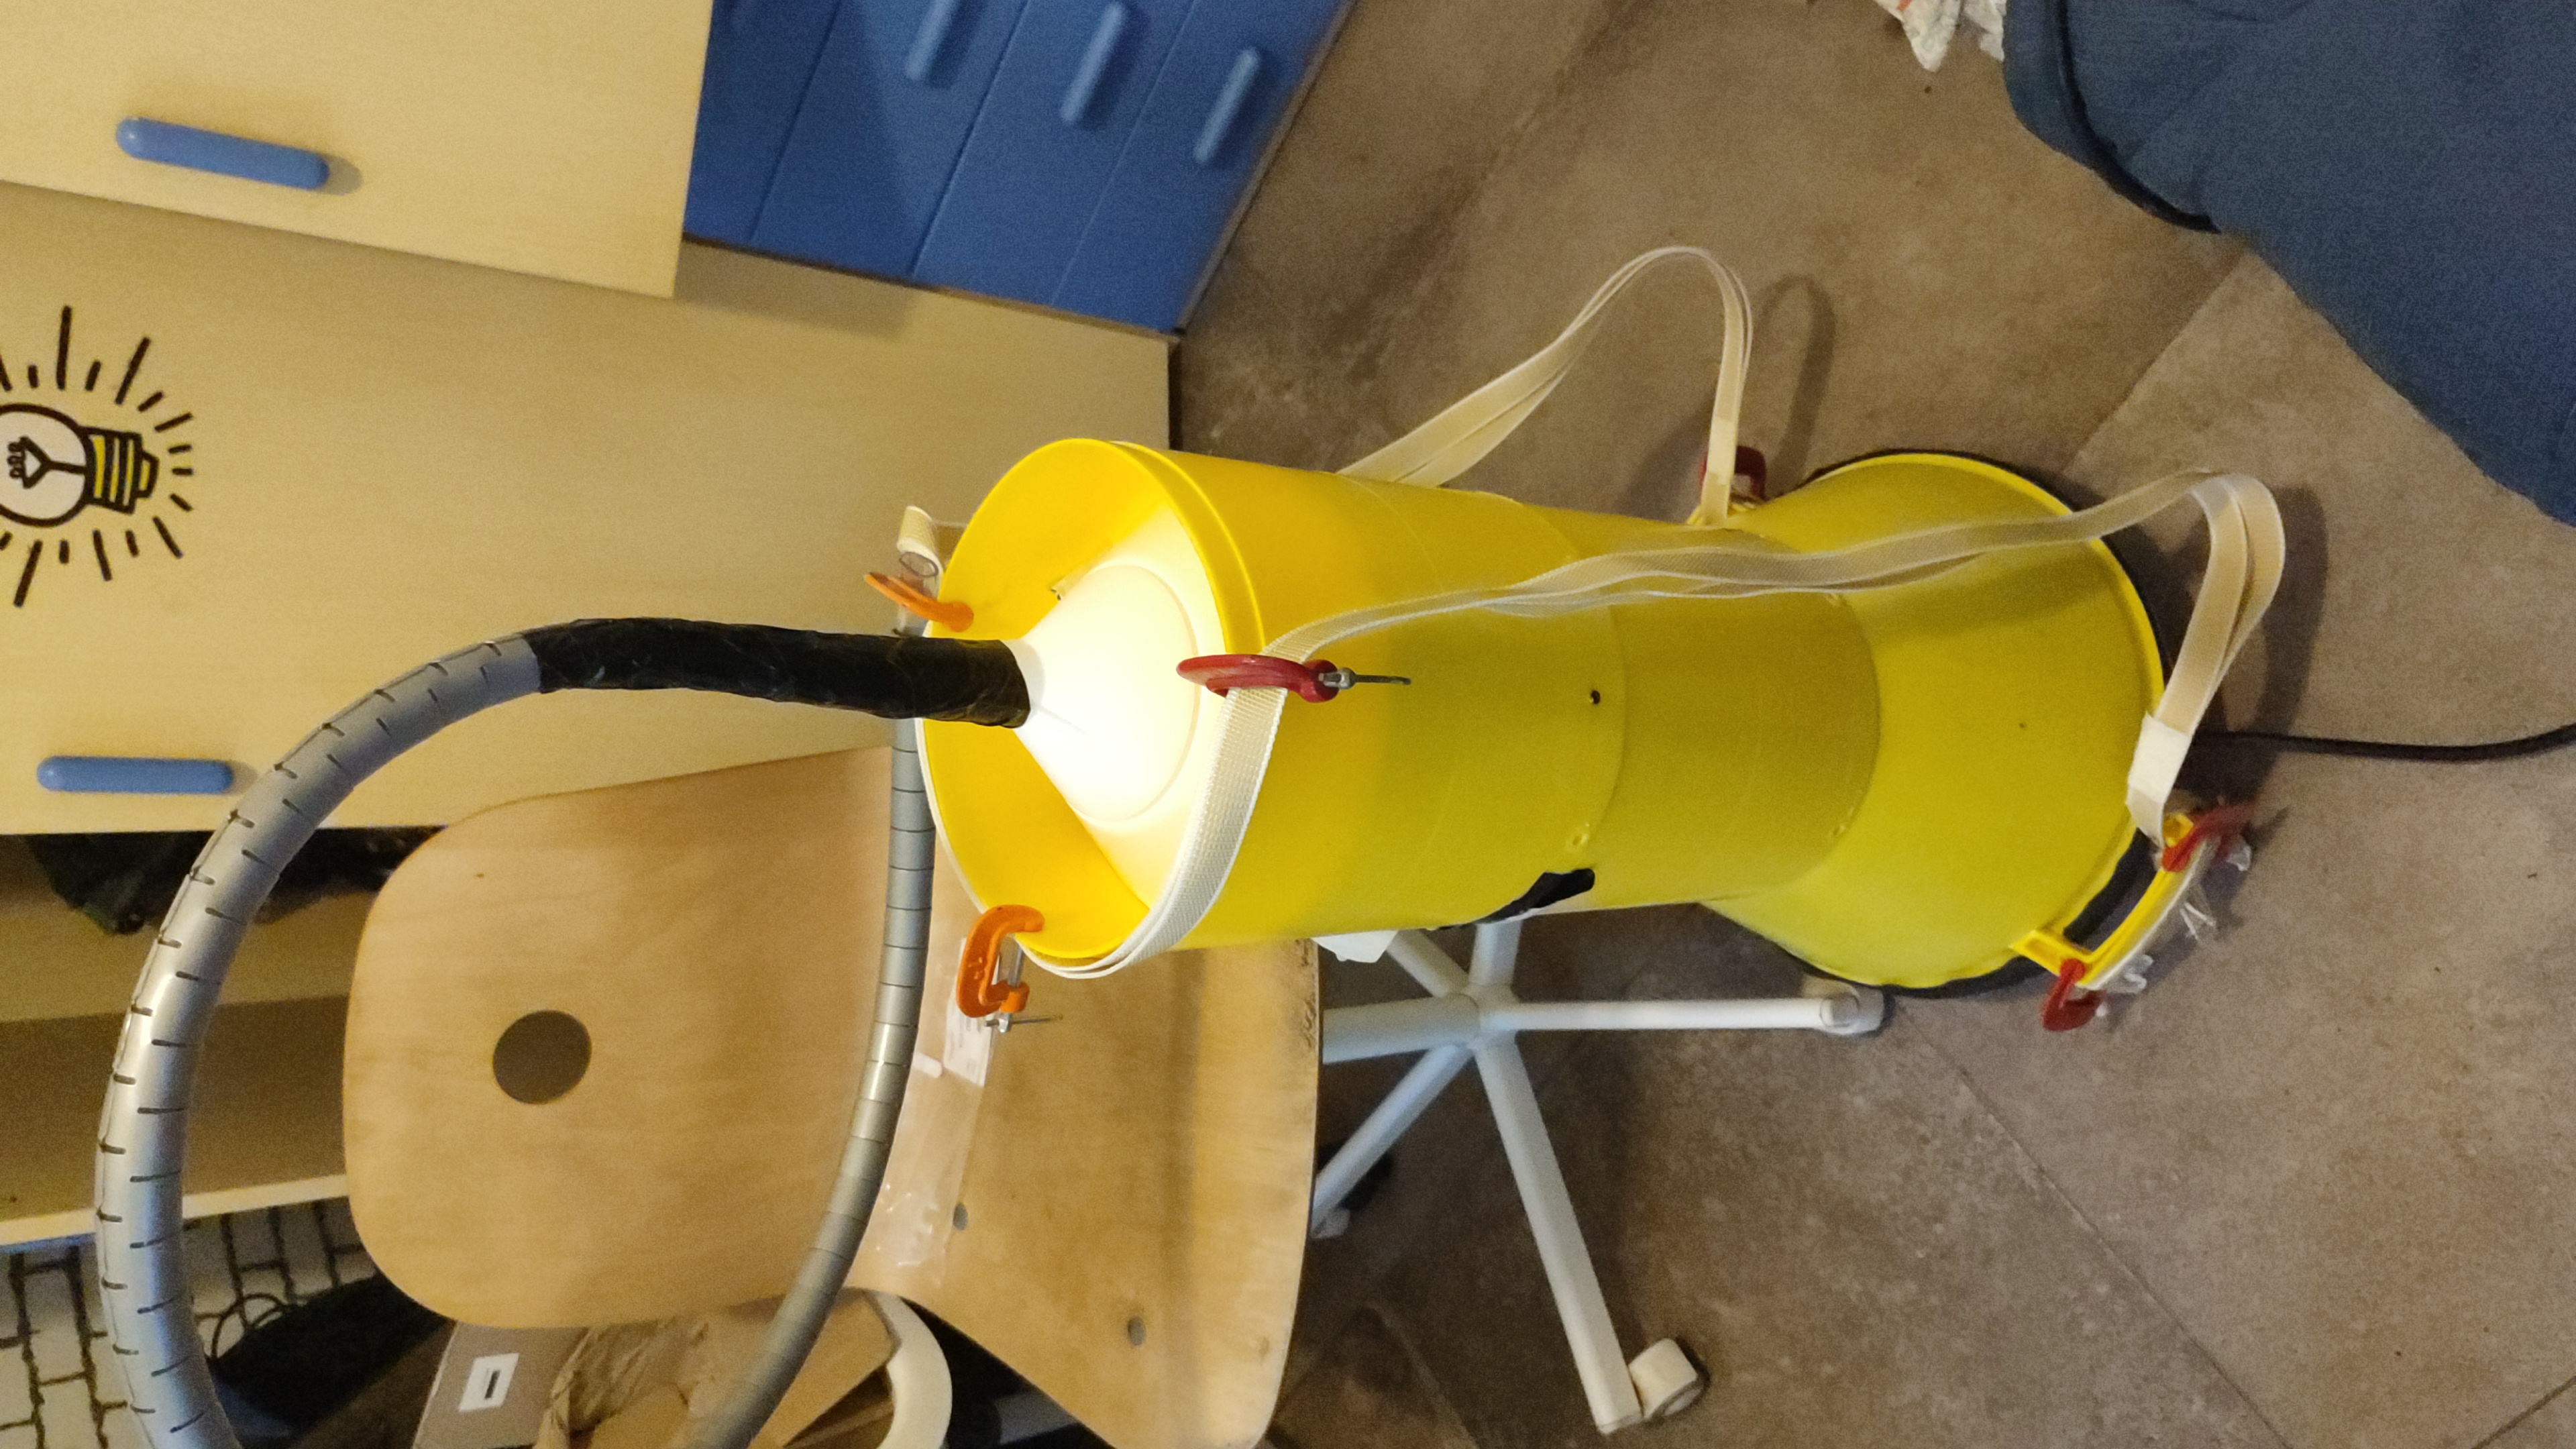
\includegraphics[width=.45\columnwidth]{Graphics/foto/1697478266898}}
\caption{Imbutone}
\label{fig:imbutone}
\end{figure}

È stato possibile trovare in commercio un imbuto di plastica con un diametro nominale di 22cm che riesce ad incastrarsi perfettamente all’interno del cilindro dell’imbutone [Fig. \ref{fig:imbutone}].

Per inserire l’altoparlante all’interno del cilindro dell’ imbutone è stato realizzato un anello in legno [Fig. \ref{fig:imbutone}].

L’anello è stato fissato alla struttura tramite quattro viti di legno. In tal modo è stato possibile inserire l’altoparlante nel cilindro poggiandolo sull’anello di legno e fissando anche esso con delle viti [Fig. \ref{fig:imbutone}]. Per non correre il rischio di fuoriuscite di pressione del flusso dalla parte dell’altoparlante, l’anello di legno è stato sigillato con del silicone da ambedue le parti.

La posizione dell’altoparlante è stata scelta tramite una serie di prove di suono empiriche con lo scopo di trovare la migliore risonanza.

È stato necessario insonorizzare internamente tutta la parte inferiore dell’imbutone. A tal proposito è stato realizzato un coperchio in legno corrispondente esattamente al disegno della faccia posteriore dell’imbutone, manici compresi [Fig. \ref{fig:imbutone}].

Sia la parete interna della parte bassa dell’imbutone, che la facciata interna del coperchio di legno sono state rivestite con una spugna insonorizzante ondulata [Fig. \ref{fig:imbutone}].

Per far ciò è stato necessario disegnare geometricamente lo sviluppo del tronco di cono, equivalente a un arco di corona circolare e ritagliarlo sulla spugna insonorizzante [Fig. \ref{fig:imbutone}]. È stato più agevole insonorizzare la parte di cilindro intermedia tra l’altoparlante e il tronco di cono, in quanto essa corrispondeva a un rettangolo di cui era facile calcolare la base e l’altezza.

Per far aderire il tappo di legno all’imbutone sono stati applicati alle maniglie quattro morsetti.
Un tubo di gomma, incastrandosi da entrambi gli estremi, collega la parte terminale dell’imbuto di diametro $22 cm$ con il flauto. Il collegamento del tubo con l’imbuto è stato rinforzato con del nastro telato. Il tubo di plastica essendo soggetto a piegamenti è stato rivestito con una canalina passa cavi per mantenere una forma curvilinea.

La pressione generata dal sistema ha consentito di reinserire il tappo all’interno della testata  rimuovendo l’asta filettata  in modo da lasciare libero un foro per il passaggio dell’aria. La presenza del tappo ha consentito di poter mantenere pressoché inalterato  il rapporto tra le ottave.

Infine delle cinte da serranda sono state applicate a tutta la struttura in modo tale da formare due bretelle che consentono all’interprete di avere stabilmente il prototipo sulle spalle. [Fig. \ref{fig:imbutone}]

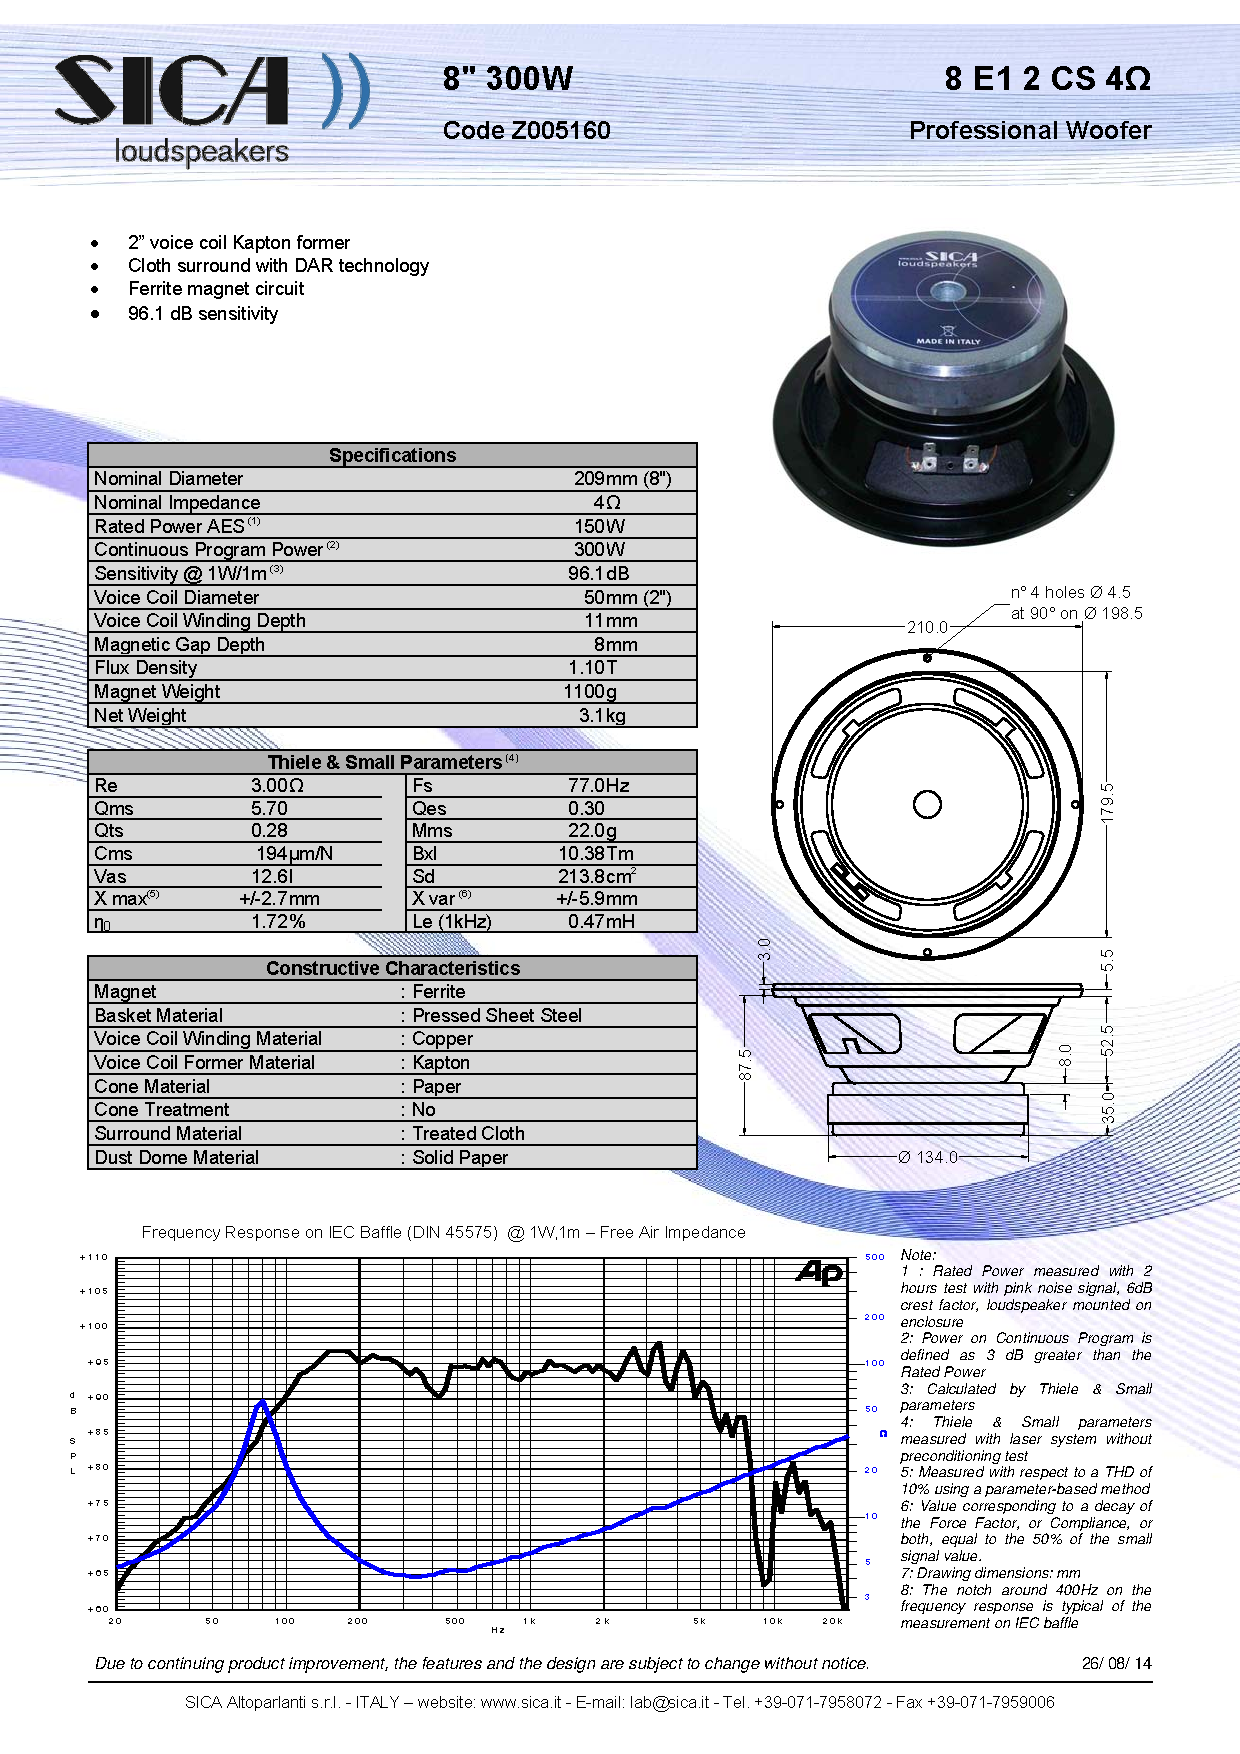
\includepdf[pages=-]{Graphics/foto/Z005160C.pdf}
